\chapter{Blank Study Templates}
\label{app:blank_templates}

This appendix contains the blank versions of all study instruments used in the pilot validation study. These templates were used to produce the completed materials in Appendix~\ref{app:completed_materials}.

A note on the Informed Consent Form (ICF): the ICF was submitted with the original protocol to the Bucknell University Institutional Review Board (Protocol \#2526-025) and reflects the study design as initially proposed. The protocol was refined before data collection began; the key differences between the ICF and the executed protocol are as follows. First, phase durations were adjusted: Training was planned at 15 minutes, the Design Challenge at 30 minutes, the Live Trial at 10 minutes, and the Debrief at 5 minutes, rather than the 10/20/15/15-minute allocations stated in the ICF. Second, screen recording during the design phase was not implemented, as the DFS is scored from the exported project file rather than from screen footage. Third, the live trial was conducted with the researcher serving as the test subject rather than a recruited student volunteer, as discussed in Chapter~\ref{ch:evaluation}. The ODS, DFS, ERS, and SUS templates reflect the protocol as executed.

\medskip
\noindent\textbf{Contents of this appendix, in order:} ODS, DFS, ERS, SUS, ICF

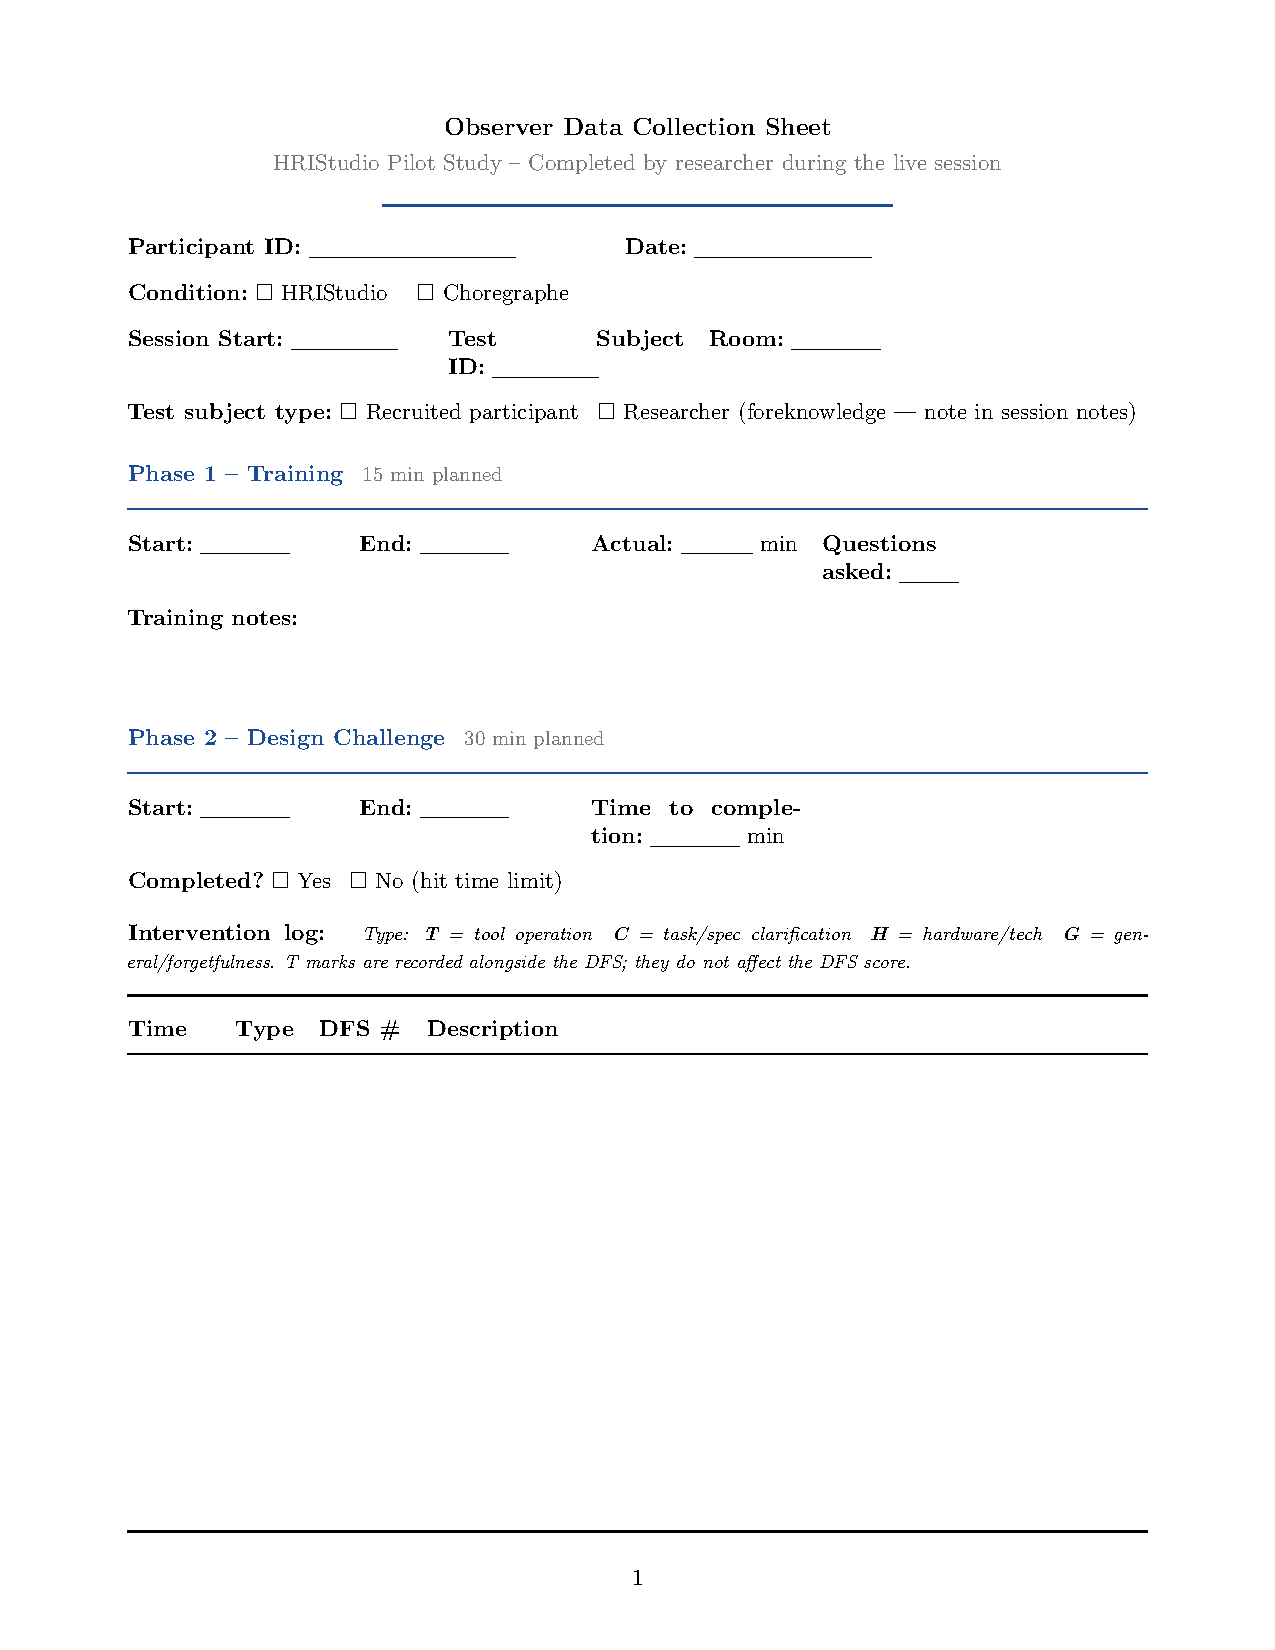
\includepdf[pages=-,pagecommand={}]{pdfs/templates/ODS-Template.pdf}
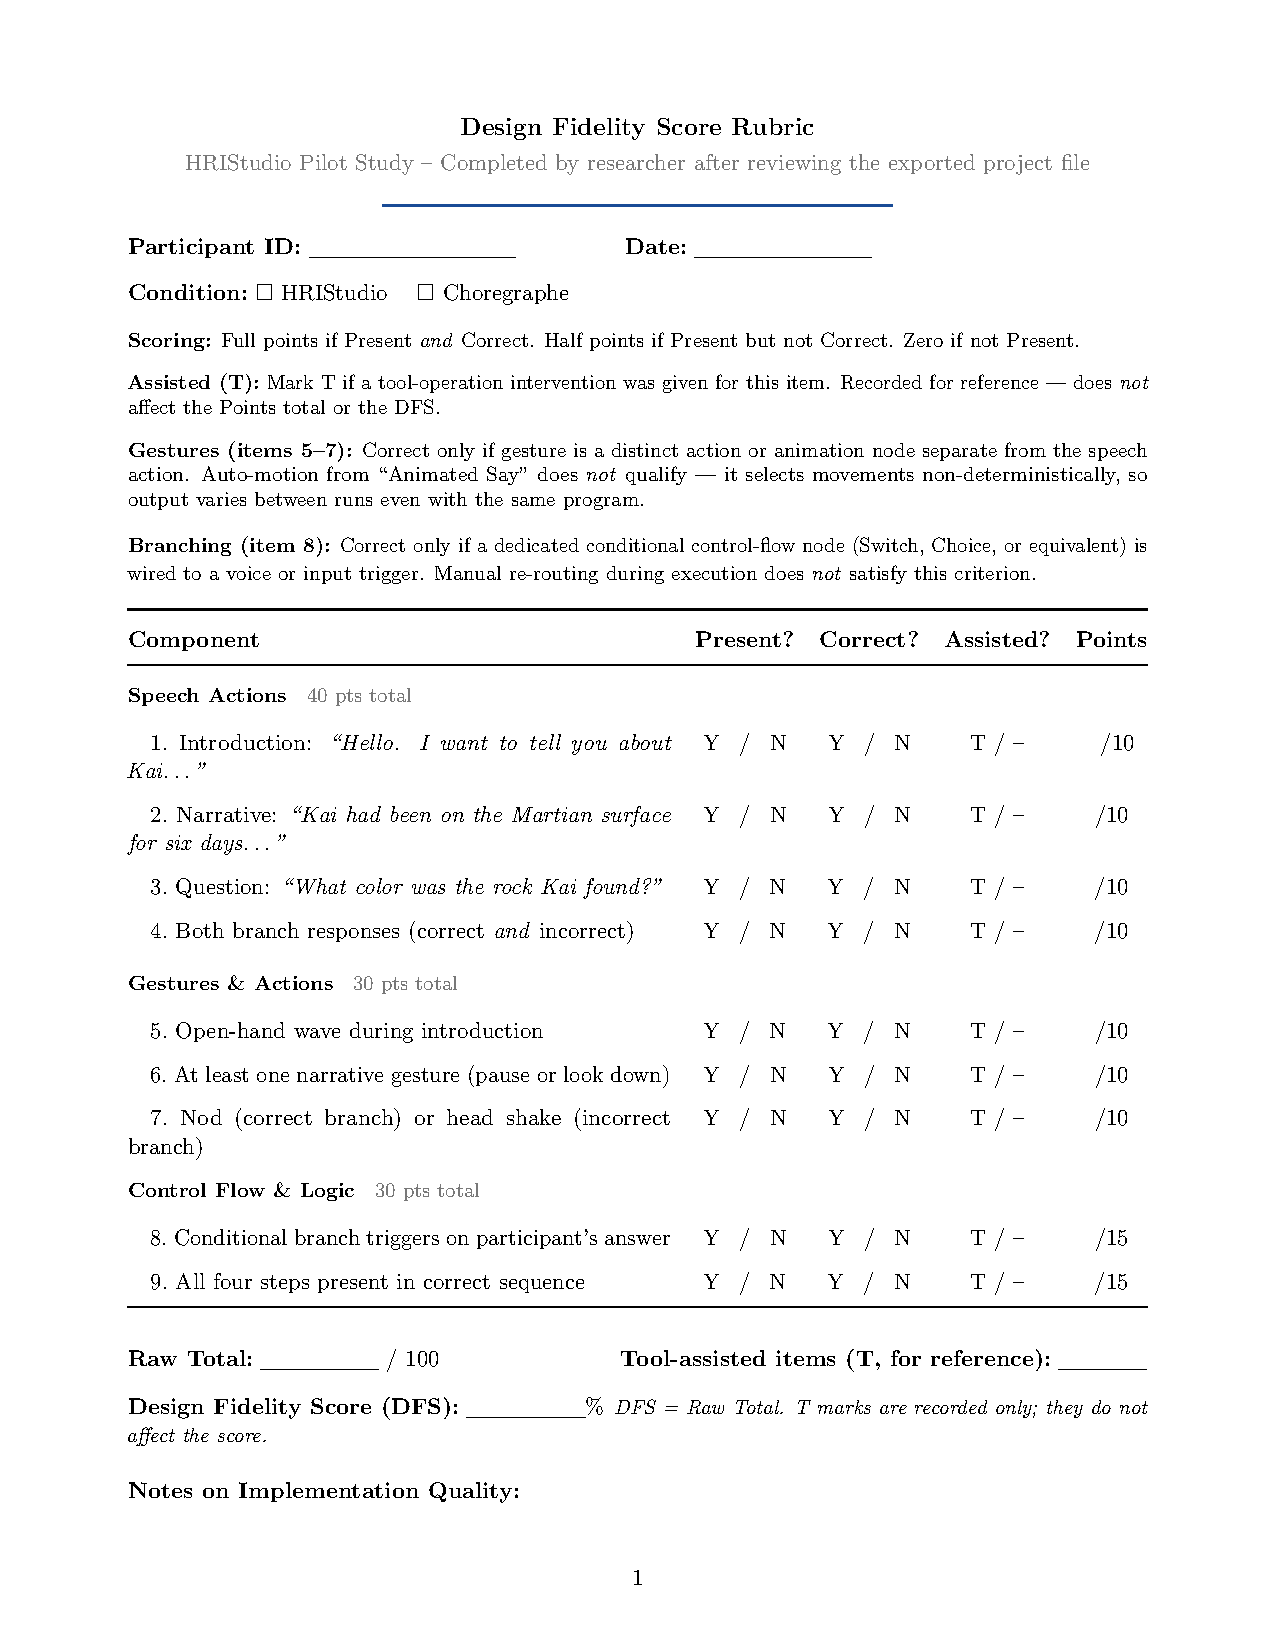
\includepdf[pages=-,pagecommand={}]{pdfs/templates/DFS-Template.pdf}
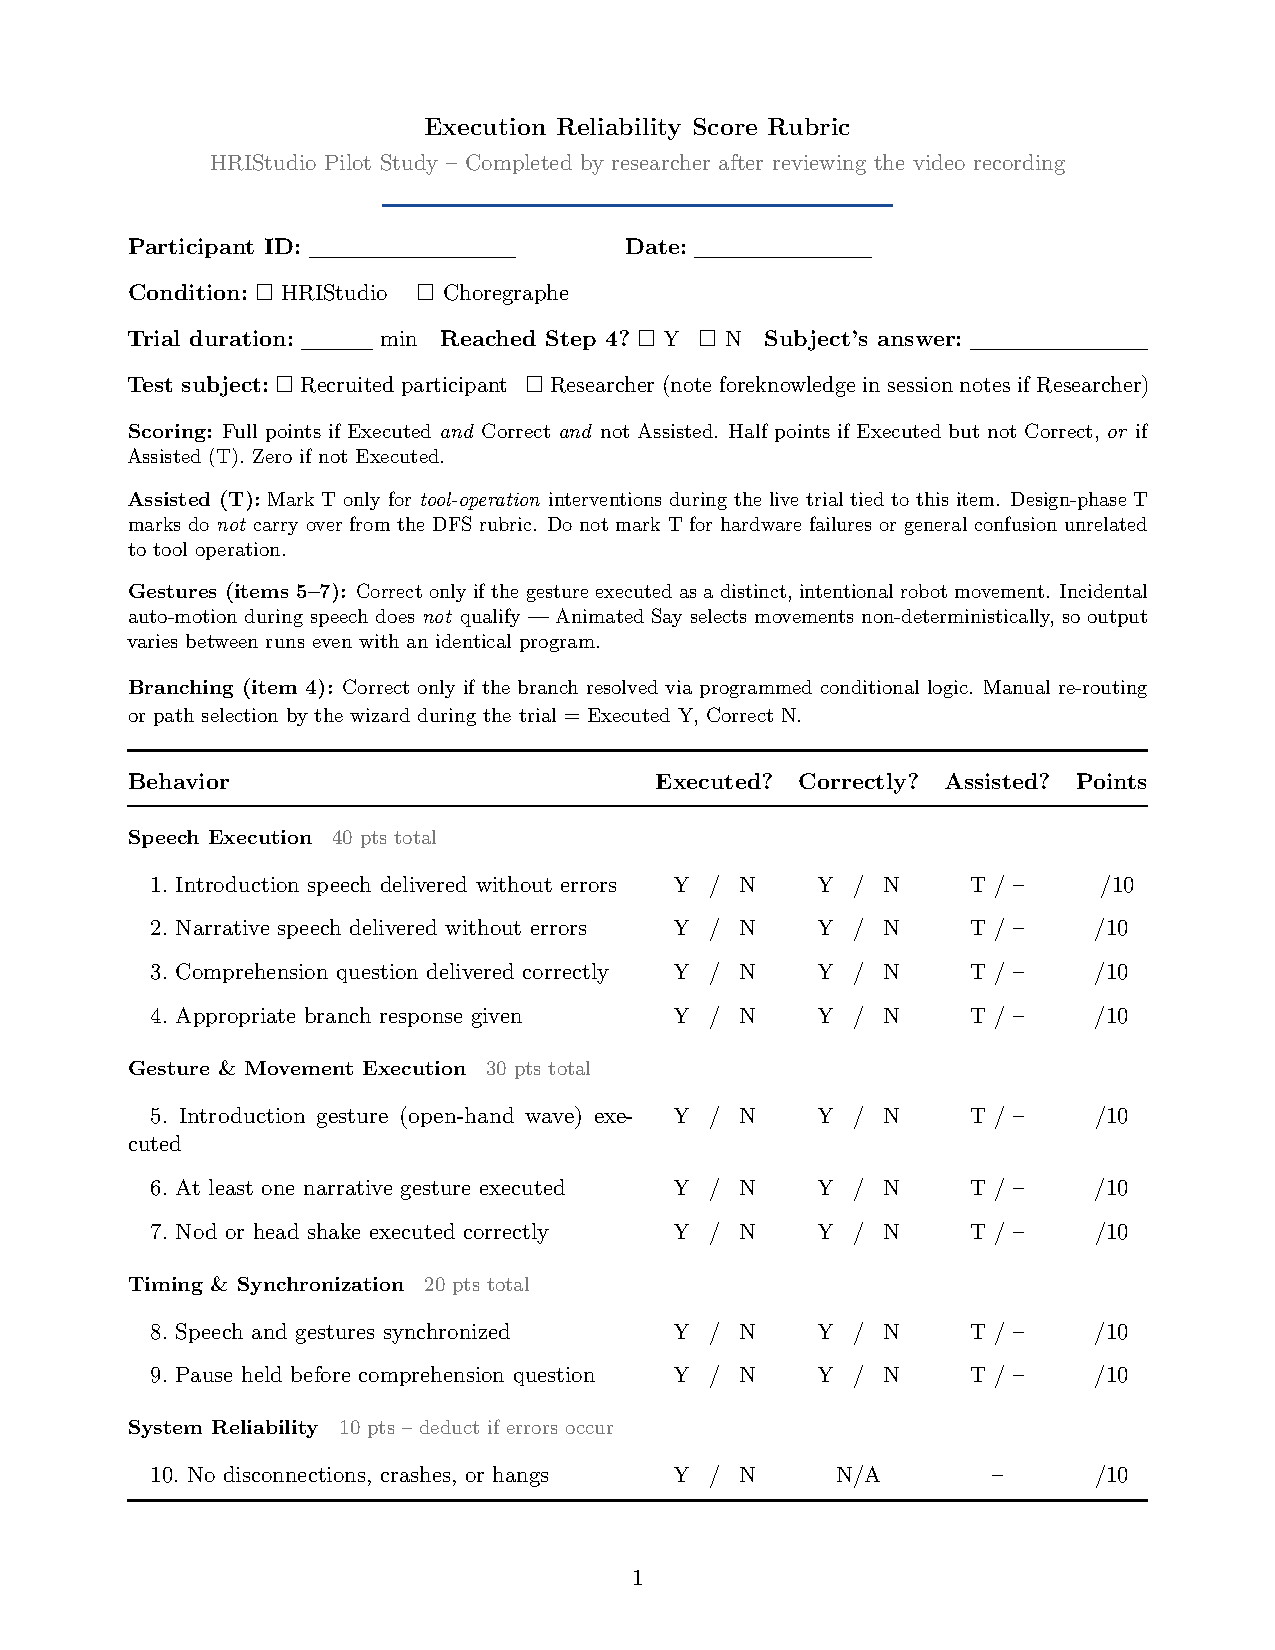
\includepdf[pages=-,pagecommand={}]{pdfs/templates/ERS-Template.pdf}
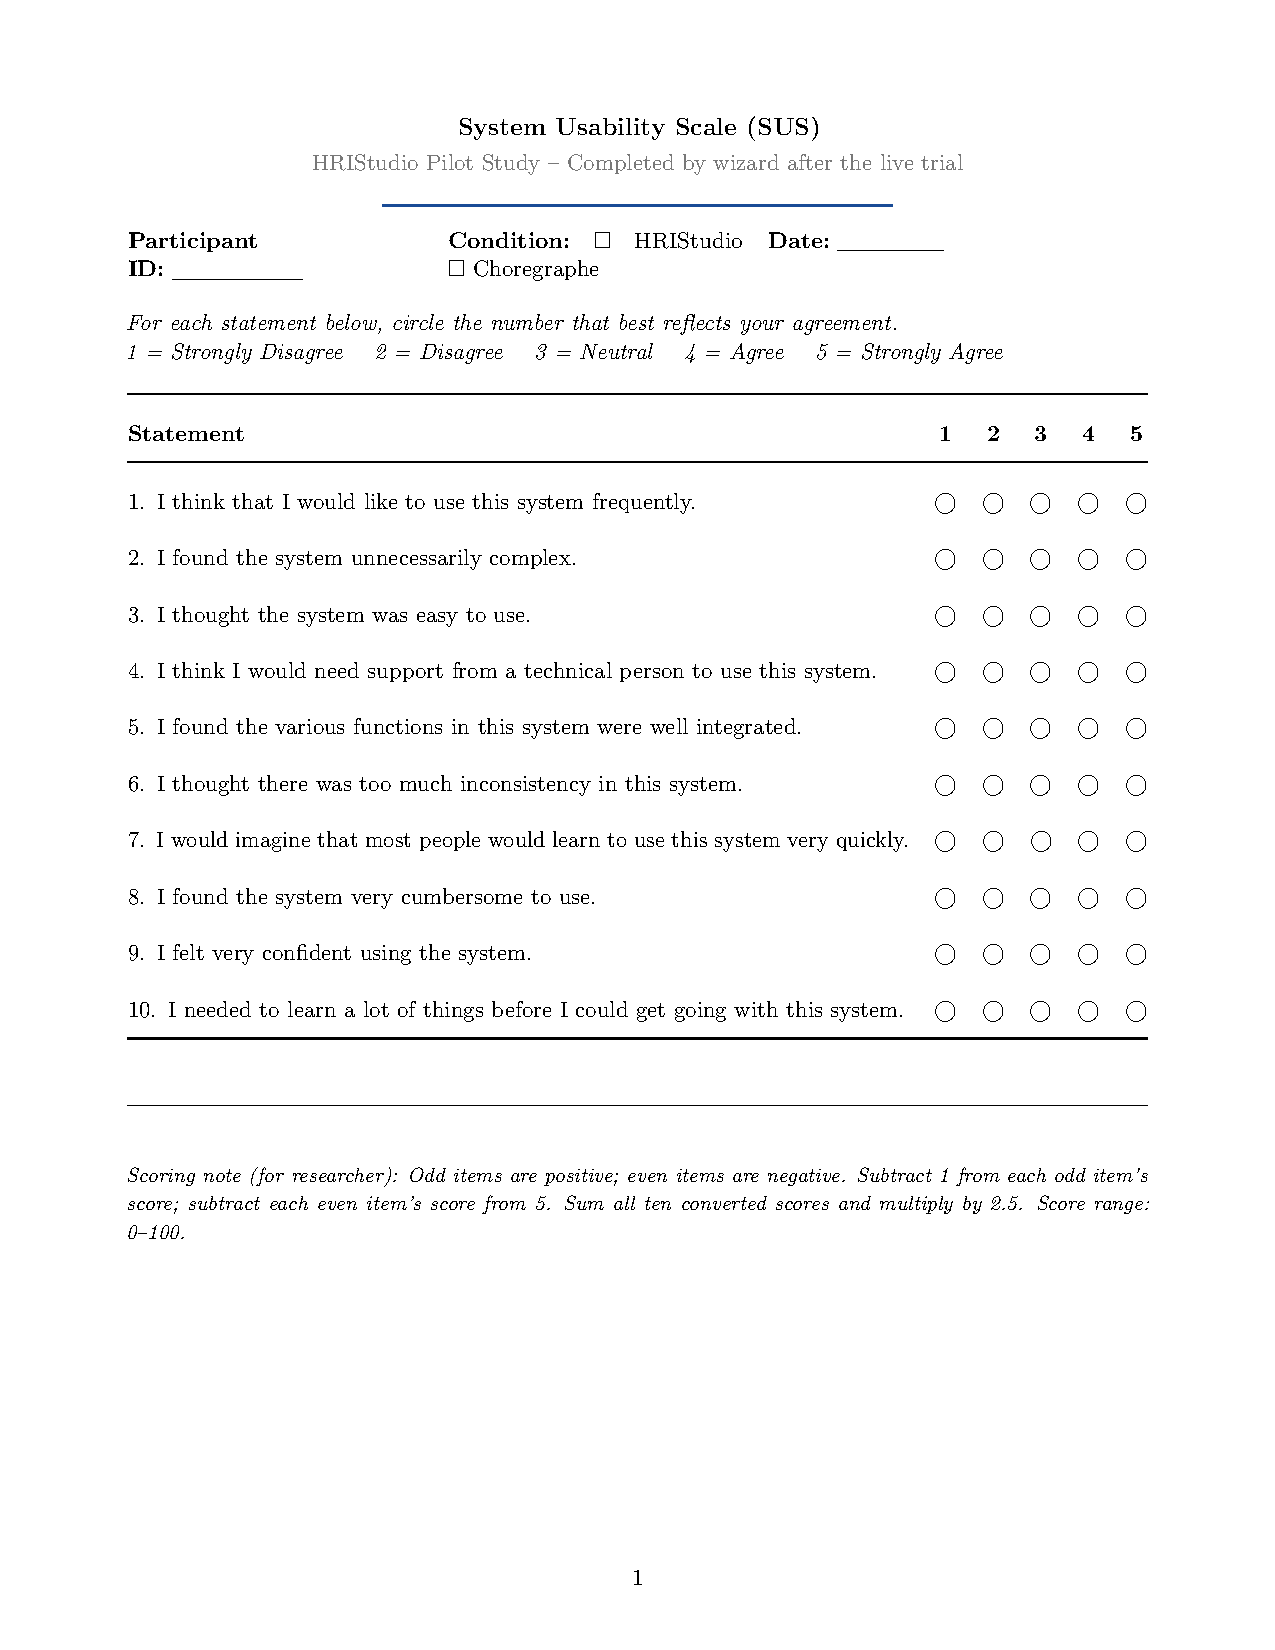
\includepdf[pages=-,pagecommand={}]{pdfs/templates/SUS-Template.pdf}
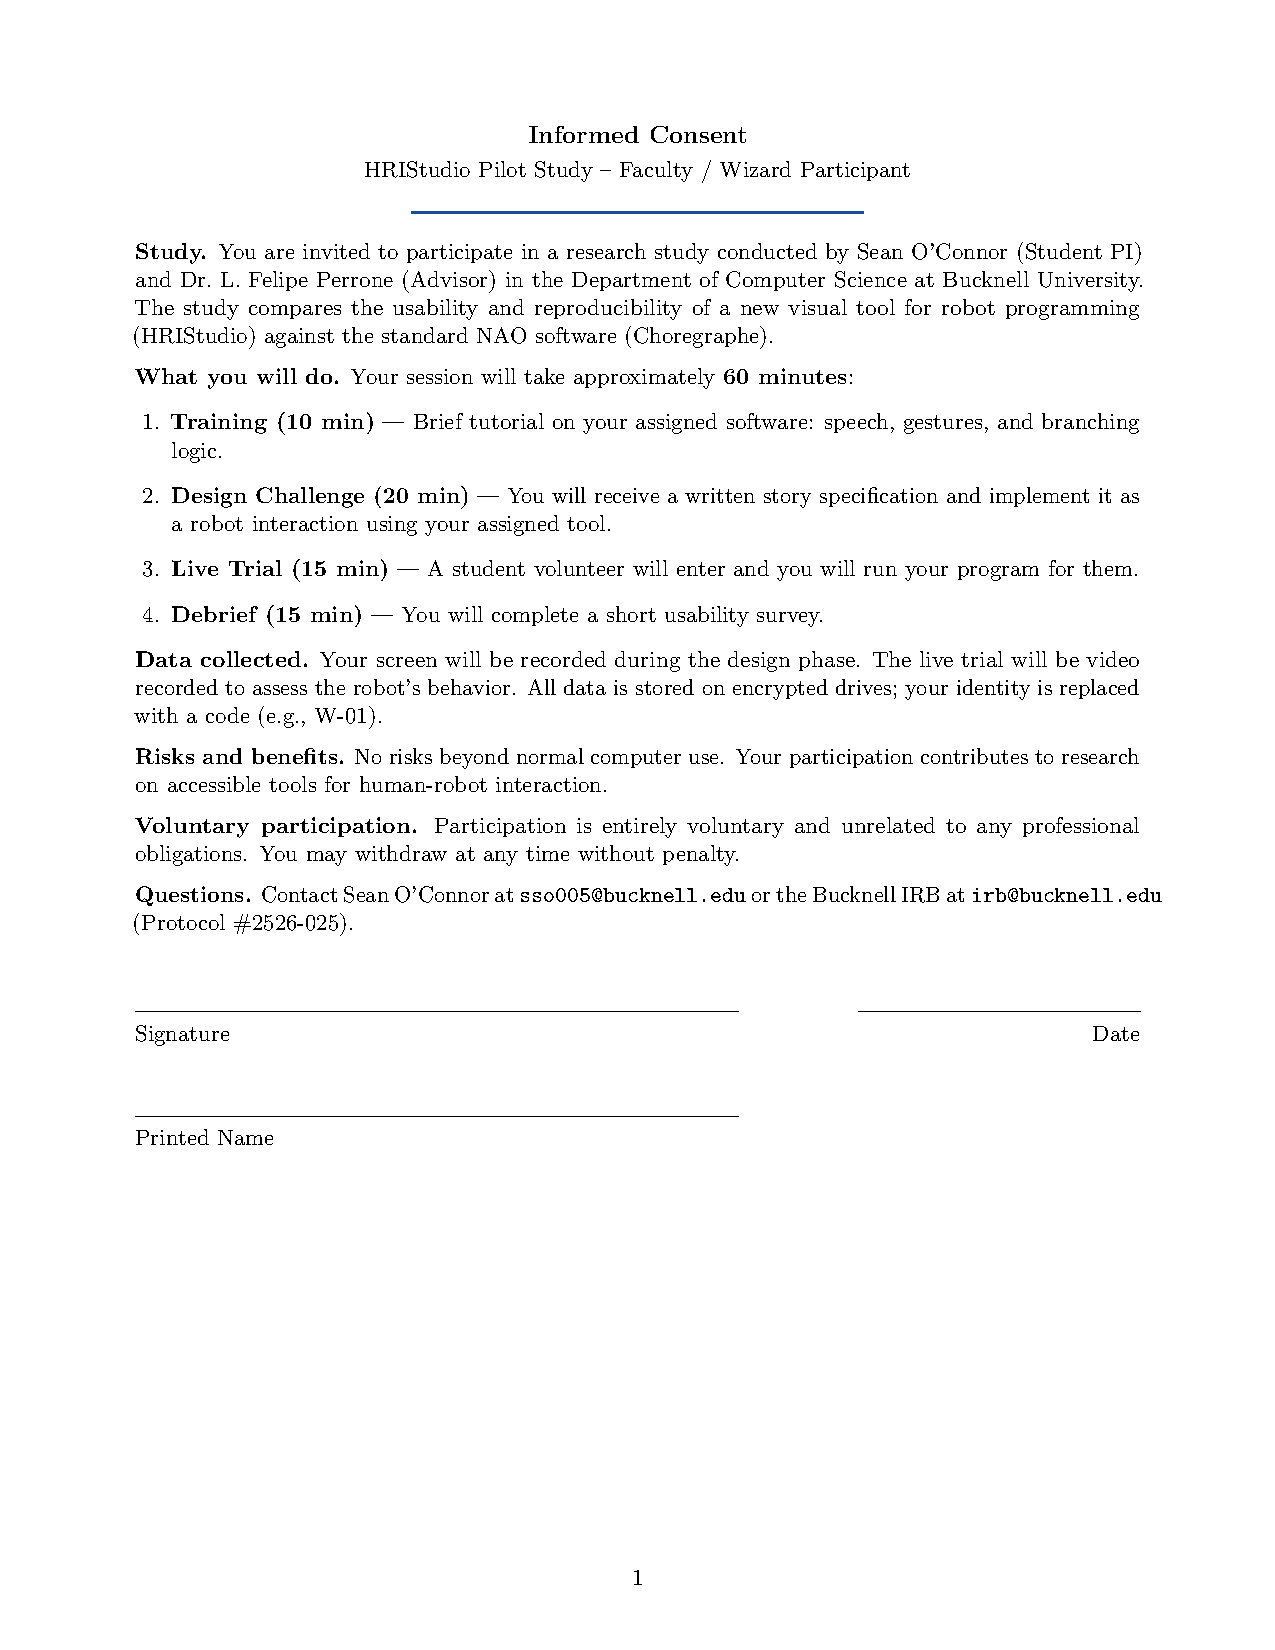
\includepdf[pages=-,pagecommand={}]{pdfs/templates/ICF-Template.pdf}
